% siminos/CLE/movingFrames.tex
% $Author: siminos $ $Date: 2009-12-19 02:59:14 +0100 (Sat, 19 Dec 2009) $

The \mframes, introduced by G. Darboux and systematized by
\'E. Cartan\rf{CartanMF}, can be thought of as generalization
of the Frenet-Serret co-moving frame.
\ES{Fels and Olver claim that ``a moving
frame as an equivariant map from a manifold to a Lie group''
is exactly \emph{their} interpretation of \mframes\
so I've dropped this: The notion of a {\em moving frame}
as a map from a manifold to a Lie group was introduced
by Cartan\rf{CartanMF}.}
Fels and Olver\rf{FelsOlver98,FelsOlver99} reinterpret a moving
frame as an equivariant map from a manifold to a Lie group.
Moving frames are then used to compute functionally independent
fundamental invariant bases for general group actions in relation
to general equivalence problems. `Fundamental' here means that
they can be used to generate all other invariants. For an
introduction to the method, specific to the interpretation
in \refrefs{FelsOlver98,FelsOlver99}, we recommend Olver's
pedagogical monograph\rf{OlverInv}. Our presentation draws
from the formulation of Fels and Olver but here we attempt
to establish an explicit connection to symmetry reduction for
differential equations. Specifically, we do not
focus in the explicit determination of nonlinear invariant functions
as in \refref{FelsOlver98,FelsOlver99} but rather on implementation
of a moving frame transformation as a linear, and therefore
efficient, geometrical operation.

The main idea behind \mframes\ is that we can, at least locally,
map each point along any solution $\ssp(\tau)$ to a unique
representative $\sspRed(\tau)$ of the associated
group orbit equivalence class, by a suitable rotation
\beq
\ssp(\tau) = \LieEl(\tau) \, \sspRed(\tau)
\,.
\ee{EquiTraj}
Equivariance implies the two points are equivalent.
In the `\mframes' the \reducedsp\ representative $\sspRed$
of a group orbit equivalence class is picked by slicing across the group orbits
by a fixed hypersurface.
%
%%%%%%%%%%%%%%%%%%%%%%%%%%%%%%%%%%%%%%%%%%%%%%%%%
% (b) ESunrot computed by PCunrot.nb, then hand-drawn
% by dasbuch/book/FigSrc/xfig/PCunrot.fig
% then branched to dasbuch/book/FigSrc/xfig/ESunrot.fig
\begin{figure}[ht] \label{fig:ReducTraj}
\begin{center}
(\textit{a})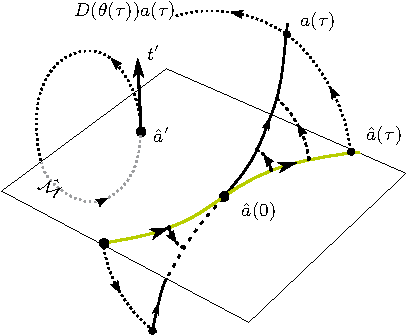
\includegraphics[width=0.43\textwidth]{ReducTraj1}
~~~~(\textit{b})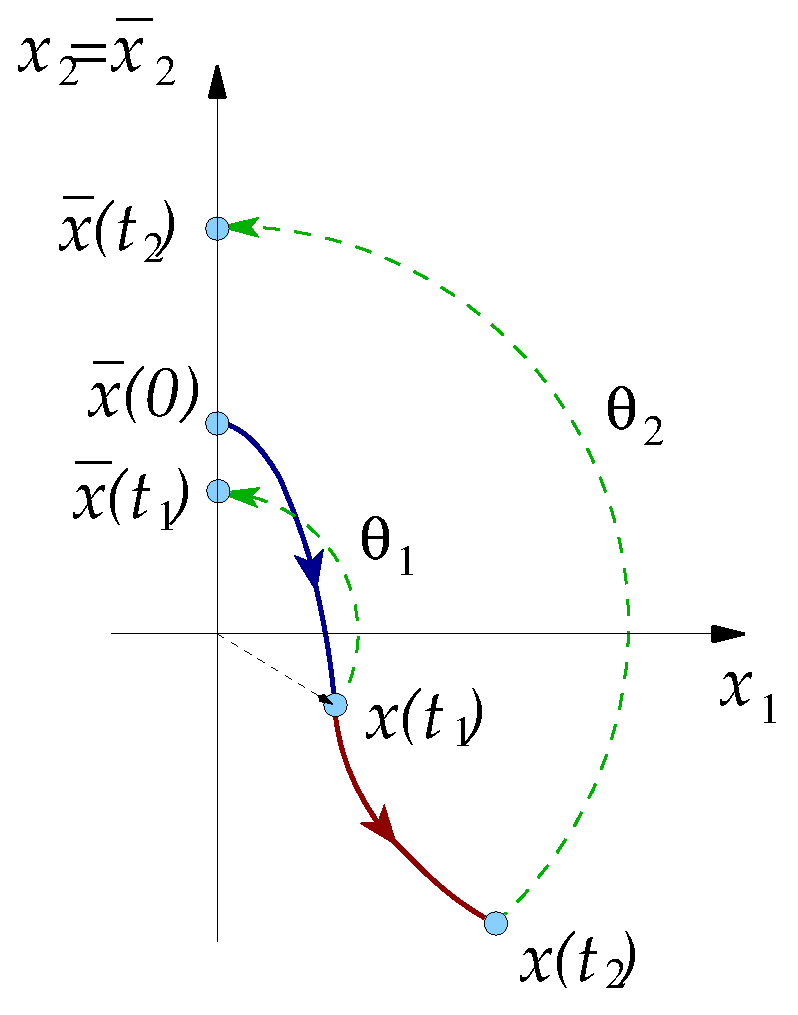
\includegraphics[width=0.43\textwidth]{ESunrot}
\end{center}
\caption{
(a)
\Slice\ \pSRed\ is a hyperplane \refeq{PCsectQ} which intersects
all
group orbits (indicated by dotted lines here) in an open
neighborhood of the slice-fixing point $\slicep$. The full
\statesp\ trajectory $\ssp(t)$ and the \reducedsp\
trajectory $\sspRed(t)$ belong to the same group orbit
$\pS_{\ssp(t)}$ and are equivalent up to a group rotation
$\LieEl(t)$.
~~~(b)
\Mframes\ for a flow $\SOn{2}$-equivariant under
\refeq{CLfRots} with \slice\ through $\slicep=(0,1,0,0,0)$,
group tangent $\sliceTan{}=(1,0,0,0,0)$. The clockwise
orientation condition restricts the \slice\ to half-hyperplane
$\sspRed_1=0,\;\sspRed_2>0$. A trajectory started on the
\slice\ at $\sspRed(0)$, evolves to a \statesp\ point with a
non-zero $\ssp_1(t_1)$. Compute the polar angle $\gSpace_1$
of $\ssp(t_1)$ in the $(\ssp_1,\ssp_2)$ plane. Rotate $\ssp(t_1)$
clockwise by $\gSpace_1$ to $\sspRed(t_1) =
\LieEl(-\gSpace_1)\,\ssp(t_1)$, so that the equivalent point
on the circle lies on the \slice, $\sspRed_1(t_1) =0$. Repeat
for all sample points $\ssp(t_i)$ along the trajectory.
}
\end{figure}
%%%%%%%%%%%%%%%%%%%%%%%%%%%%%%%%%%%%%%%%%%%%%%%%%%
%
\ES{move elsewhere: We start by describing how the
method works for a finite segment of the full \statesp\
trajectory.}

In the following it will be useful to introduce the notion of
a \emph{\slice}, an $(d-N)$-dimensional submanifold
$\pSRed\subset\pS$ such that $\pSRed$ intersects all group
orbits in an open neighborhood of $\slicep \in \pSRed$
transversally and at most once. In other words, `\slice' is
the analogue of a Poincar\'e section, but for group orbits.
As is the case for the dynamical Poincar\'e sections, in
general a single \slice\ does not suffice to intersect all
group orbits of points in \pS. Fels and Olver\rf{FelsOlver99}
call a manifold $\pSRed$ that intersects \emph{all} group
orbits a \emph{regular cross-section}, and refer to a \slice\
as a local cross-section. Here we prefer the term `slice' to
`cross-section' as the latter has a well established usage in
the physics literature. One can construct a local {\slice}
passing through any point $x\in \pS$ if the group orbits of
\Group\ have the same dimension, \ie\ away from {\fixedsp s}
of continuous subgroups of \Group, see \refref{FelsOlver99}
for details.

The simplest {\em \slice\ condition} defines a linear \slice\ as a
$(d\!-\!N)$-dim\-ens\-ion\-al hyperplane \pSRed\ normal to
the $N$ group rotation tangents $\sliceTan{a}$ at point $\slicep$:
\beq
(\sspRed - \slicep )^T \sliceTan{a} =0
    \,,\qquad
\sliceTan{a} = \groupTan_a(\slicep) = \Lg_a \, \slicep
\,.
\ee{PCsectQ}
As the group orbit will in general intersect a group orbit
more than once, for example in the case of $\SOn{2}$ in two
$\pi$-separated point we need to impose further conditions on
the slice, either in the form of inequalities or of
orientation conditions, so as to ensure unique intersection.
This restriction is rather arbitrary, the only requirement
being that $\pSRed$ remains a connected manifold. We
illustrate this point in \cLf\ example in
\refsect{sec:CLeMovFr}.

For group orbits intersected by a slice we can identify the
unique group element $\LieEl=\LieEl(\ssp)$ that rotates
$\ssp$ into the slice, $\LieEl\ssp = \sspRed \in \pSRed$. The
map that associates to a \statesp\ point $\ssp$ a Lie group
action $\LieEl(\ssp)$ is called a \emph{moving frame}.
\Mframes\ can be interpreted as a change of variables
\beq
\sspRed = \LieEl^{-1} \, \ssp
\,,
\ee{EquiTrajInvrs}
to a frame of reference in which condition \refeq{PCsectQ1}
is identically satisfied. Therefore the name `moving frame.'



As $\slicep^T \sliceTan{a} =0$ by the antisymmetry of
$\Lg_a$, the \slice\ condition \refeq{PCsectQ} fixes
$\gSpace$ for a given $\ssp$ by
    \index{post-processing}
\beq
0 = \sspRed^T  \sliceTan{a}
  %= \LieEl(\gSpace) \cdot \hat{\ssp}   \cdot \Lg \cdot \slicep
	=\ssp^T  \LieEl(\gSpace)^T \sliceTan{a}
\,,
\ee{PCsectQ1}
where $\LieEl^T$ denotes the transpose of $\LieEl$.
%    \PC{dropped ``
%    with the total shift $\gSpace(\tau)$ given by the sum
%    of stepwise rotations $\gSpace_j$.
%    }



The \mframes\ is a post-processing method; trajectories are
computed in the full \statesp, then rotated into the \slice\
whenever desired, with the \slice\ condition easily
implemented. The \slice\ group tangent \sliceTan\ \, is a given
vector, and $\LieEl(\gSpace)\,\ssp$ is
another vector, linear in $\ssp$ and a function of group
parameters $\gSpace$. Rotation parameters $\gSpace$ are
determined numerically, by a Newton method, through the \slice\
condition \refeq{PCsectQ1}.


Through the definition of a moving frame map, a \slice\ is
locally identified with $\pS/\Group$, in an open
neighborhood of $\slicep$. As is the case for the dynamical
Poincar\'e sections, in general a single \slice\ does not
suffice to reduce $\pS \to \pS/\Group$ globally as
for general group actions one cannot expect the group orbit
of any point in $\pS$ to intersect a given slice.

How does one pick a \slice\ point $\slicep$? A generic point
$\slicep $ not in an invariant subspace (on the \cLe\ $z$
axis, for example) should suffice to fix a \slice.
% for example a point on an \reqv\ group orbit,
% $\slicep  = \ssp_{\REQV{}1}$.
The rules of thumb are much like the ones for picking
Poincar\'e sections. The intuitive
idea is perhaps best visualized in the context of fluid
flows. Suppose the flow exhibits an unstable coherent
structure that --approximately-- recurs often at different
spatial dispositions. One can fit a `template' to one
recurrence of such structure, and describe other recurrences
as its translations. A well chosen \slice\ point belongs to
such dynamically important equivalence class (\ie, group
orbit).
% We shall show in \refsect{sect:MovFrameODE} that
We discuss, in the context of our \cLe\ example, some simple slice fixing
choices in \refsects{s:cleCoordSlice}{s:mfReqb}.


\section{\label{sec:CLeMovFr}An example: Moving frame for \CLe}

In case of \cLe\ we can, due to equivariance, rotate any
slice point so that it is written as
$\slicep=(0,\,\slicepComp{x}{1},\,\slicepComp{y}{1},\,\slicepComp{y}{2},\,\slicepComp{z}{})$.
The group orbit tangent then becomes
$\sliceTan{}=(-\slicepComp{x}{2},\,0,\,-\slicepComp{y}{2},\,\slicepComp{y}{1},\,0)$
and slice condition \refeq{PCsectQ1} leads to
    \PC{Emphasize; the most genral form of a linear slice condition for
    \cLe. The point of my rescaling was to show that one needs only 2 numbers,
    not three ($\slicepComp{x}{1},\,\slicepComp{y}{1},\,\slicepComp{y}{2}$)
    to fix the slice. Was I wrong?
    \\
    make `coordinate slice' (stupid name) a `linear slice' or `hyperplane slice'
    everywhere.
    }
\beq
  \theta=\tan^{-1}\frac{\slicepComp{x}{2}x_1+\slicepComp{y}{2}y_1-\slicepComp{y}{1}y_2}
			  {\slicepComp{x}{2}x_2+\slicepComp{y}{1}y_1+\slicepComp{y}{2}y_2}\,.
\ee{cLeMF}
To ensure a unique intersection with the slice we have to further restrict $\pSRed$
by choosing a representative out of the two group orbit points that intersect the slice.
We can impose an orientation condition, for example choosing the angle that
results in the smallest clockwise rotation. Another choice is to pick as group
orbit representative the point that is at minimum distance from $\slicep$. Or we
can define our inverse tangent function $\tan^{-1}\frac{b}{a}$ so that it distinguishes quadrants
in the $a-b$ plane.
We have found that all three conditions work equally well, resulting in the same image dynamical
system.

We observe that \refeq{cLeMF}, is undefined when
\begin{subequations}\label{cLeMFsing}
  \begin{align}
    \slicepComp{x}{2}x_1+\slicepComp{y}{2}y_1-\slicepComp{y}{1}y_2 &=0 \label{cLeMFsingOnSlice}\cont
    \slicepComp{x}{2}x_2+\slicepComp{y}{1}y_1+\slicepComp{y}{2}y_2 &=0 \label{cLeMFsingPerpTan}\,.
  \end{align}
\end{subequations}
are both satisfied. We will refer to this $3$-dimensional linear subspace as the \emph{\sset} of the moving
frame associated with \refeq{cLeMF}\ES{I follow Gilmore, he uses the term for singularities arising in Hilbert basis
transformation problems.}. Condition \refeq{cLeMFsingOnSlice} implies that point \ssp\ is already
on the slice, $\ssp^T\slicep=0$. Condition \refeq{cLeMFsingPerpTan} implies that the group tangent
at point \ssp\ is perpendicular to group tangent at slice fixing point,
$\groupTan{}(\ssp)^T\sliceTan{}=-\ssp^T\slicep=0$, where we have used the antisymmetry of $\Lg$.
It would appear that such a singularity in the moving frame transformation does not affect us,
since \ssp\ that satisfy \refeq{cLeMFsing} are already on the \slice. The problem lies on the fact
that the limit of \refeq{cLeMFsing} as we approach the \sset\ does not exist.
For instance, consider points for which \refeq{cLeMFsingPerpTan}
holds; as we approach the singularity with positive values of the numerator in \refeq{cLeMF}
we have $\theta=\pi/2$, while for negative values $\theta=-\pi/2$. A $\pi$-jump occurs as
we cross the \sset. In general such crossings are expected to occur since the \sset\ is not
flow invariant. Even worse, the singularity distorts the way trajectories
are mapped onto the slice, even if they merely approach it rather than crossing it, as we
will see in the next two sections.

\subsection{\label{s:cleCoordSlice}Linear {\slice s} and explicit invariants}

We now show how a particular choice of slice point enables us
to express for the transformation to invariant variables in a
simple analytic form.

We place the \slice\ point in one of the linearly irreducible
subspaces of $\SOn{2}$ action \refeq{CLfRots}, for instance
$\slicep=(0,-1,0,0,0)$. The group-tangent at the \slice\
point is then $\sliceTan{}=(1,0,0,0,0)$ and the slice fixing
condition is
\beq
    \overline{x}_1 = x_1 \cos\gSpace - x_2 \sin\gSpace = 0
\,.
\ee{cLeCoordSlice}
The clockwise orientation condition restricts the \slice\ to half-hyperplane
$\overline{x}_1=0,\;\overline{x}_2\ge 0$.
\ES{Predrag dropped this but I disagree: ``In general, when a \slice\ $\pSRed$ is defined through
relations of the form $\overline{x}_i=0$, $i=1,\ldots,N$ then
we call $\pSRed$ a \emph{coordinate \slice}.'' I don't think we can get away
with calling them ``linear slices'', all slices defined through \refeq{PCsectQ}
are linear.}

Solving \refeq{cLeCoordSlice}
for the polar angle $\gSpace$ in $(\ssp_1,\ssp_2)$ we get
\beq
  	\gSpace=\tan^{-1}({x_1}/{x_2})
\,.
\ee{cLeCoordTheta}
The transformation that rotates $\ssp$ clockwise by $\gSpace$
to $\overline{\ssp} = \LieEl(\gSpace)\,\ssp$ onto the \slice\ is found by inserting
\refeq{cLeCoordTheta} into the expression for the action of \SOn{2}
on $\ssp$,
\bea
 	\overline{x}_1 &=& x_1 \cos\gSpace - x_2 \sin\gSpace
        \,,\quad
	\overline{x}_2  =  x_1 \sin\gSpace + x_2 \cos\gSpace
                    \label{eq:CLEexplSO2a}\\
	\overline{y}_1 &=& y_1 \cos\gSpace - y_2 \sin\gSpace
        \,,\quad
	\overline{y}_2 = y_1 \sin\gSpace + y_2 \cos\gSpace
                    \nnu
\eea
yielding the transformations in analytic form:
\bea
	\overline{x}_2 &=&  r_1 = \sqrt{x_1^2+x_2^2}
                \continue
	\overline{y}_1 &=& {(x_2 y_1-x_1 y_2)}/{r_1}
                \,,\quad
	\overline{y}_2 \,=\, {(x_1 y_1+x_2 y_2)}/{r_1}
                \continue
	\overline{z} &=& z\,.
	\label{eq:invLaser}
\eea
This transformation rotates point $\ssp$ into the slice point
$\sspRed$. Alternatively, they can be viewed as providing
invariant variables on which to project dynamics, as we did
in Hilbert basis case. Note the relation to the invariant
polynomials \refeq{eq:ipLaser}, and observe that as the
rotational degree of freedom has been explicitly  used, the
\mframes\ requires no syzygies.

%%%%%%%%%%%%%%%%%%%%%%%%%%%%%%%%%%%%%%%%%%%%%%%%%%%%%%%%%%%%%%%%
\begin{figure}[ht]
\begin{center}
  (\textit{a})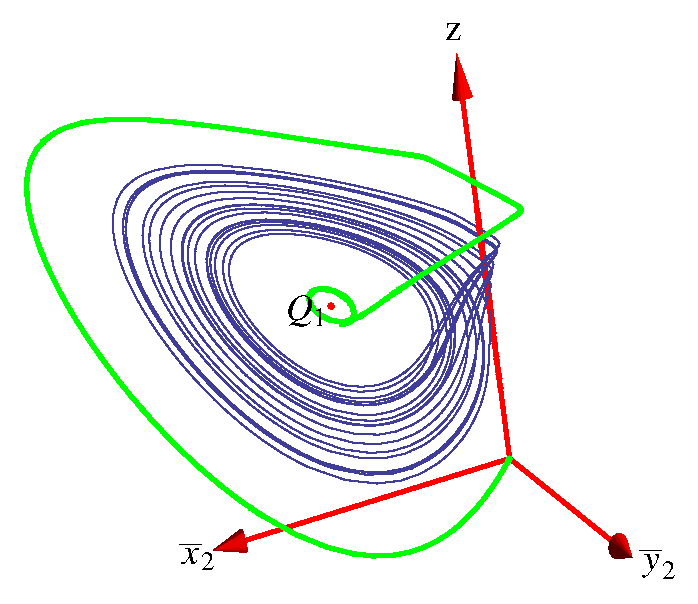
\includegraphics[width=0.35\textwidth]{CLEmfXYZ}
~~~~(\textit{b})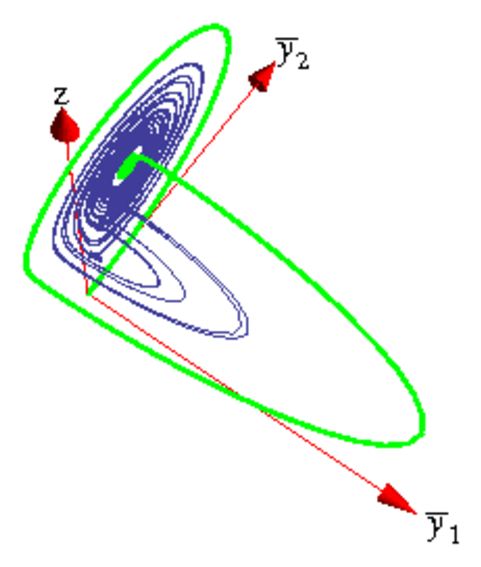
\includegraphics[width=0.35\textwidth]{CLEmfYYZ}
\end{center}
\caption{
\Statesp\ portraits of \cLe\ dynamics in \reducedsp,.
projected on invariant coordinates  \refeq{eq:invLaser}.
    }
\label{fig:CLEmf}
\end{figure}
%%%%%%%%%%%%%%%%%%%%%%%%%%%%%%%%%%%%%%%%%%%%%%%%%%%%%%%%%%%%%%%%

\ES{move elsewhere:
\refFig{fig:ReducTraj}\,(b) illustrates \mframes\ for slice fixed by
\refeq{cLeCoordSlice}.
Looks innocent, except there is nothing to
prevent a trajectory from going through $(x_1,x_2)=(0,0)$,
and what $\gSpace$ is one to use then? We can always chose a
finite time step that hops over this singularity, but in the
continuous time formulation we will not be so lucky.
}
    \PC{no reference to \refFig{fig:ReducTraj}\,(b)?}

In connection to the discussion of \refsect{sec:CLeMovFr} note that the invariants
are not well defined in the $x_1,\,x_2 \to 0$ limit.
Using $x=r_1\, e^{i\phi_1}\,,\, y=r_2\, e^{i\phi_2}$ we can write
\ES{dropped: for instance, $x_2 y_1-x_1 y_2 = r_1 r_2 \sin(\phi_1-\phi_2)$
and thus}
\beq
  \begin{split}
	  \overline{x}_2 &= r_1 \cont
	  \overline{y}_1 &= r_2\sin(\phi_1-\phi_2)\cont
	  \overline{y}_2 &= r_2\cos(\phi_1-\phi_2)\cont	
	  \overline{z} &= z\,.
	  \label{eq:invLaserPolar}
  \end{split}
\eeq
Therefore, for any given $y$ (therefore also for given $\phi_2$),
the limit of $\overline{y}$ for $x \rightarrow 0$
does not exist, as the above expression depends on the direction
on the complex $x$-plane along which we approach zero.

From a different perspective we may redefine the slice so that
$x_1=x_2=0$ is excluded, that is by $\overline{x}_1=0,\;\overline{x}_2>0$.
Then we may say that group orbits of points in the $x_1=x_2=0$
subspace fail to intersect the slice.
In \reffig{fig:CLEmf} this becomes apparent by the trajectories in reduced space being
stretched as they come closer to $x_1=x_2=0$ subspace where
transverse intersection would eventually fail. In \cLe\ example no
trajectories enter the $x_1=x_2=0$ subspace, but this is a fortuitous
event\ES{point to next section after fixing discussion there.}.

It is instructive to write \cLe~\refeq{eq:CLe} in the
variables \refeq{eq:invLaser}. This is achieved by using the
chain rule \refeq{HilbChainRl} and expressing the result in
terms of variables \refeq{eq:invLaser}. The equations now
read
\beq
\begin{split}
\dot{\overline{x}}_1 &= 0\,\\
\dot{\overline{x}}_2 &=-\sigma  \left(\overline{x}_2-\overline{y}_2 \right)\,,\\
\dot{\overline{y}}_1 &=-\overline{y}_1- \left(e+\sigma\frac{\overline{y}_1}{\overline{x}_2} \right)\overline{y}_2\,,\\
\dot{\overline{y}}_2 &=(\RerCLor -z)\overline{x}_2+\left(e+\frac{\sigma  \overline{y}_1}{\overline{x}_2}
\right) \overline{y}_1-\overline{y}_2\,,\\
\dot{z} &=\overline{x}_2 \overline{y}_2-b z\,.
\end{split}
\eeq
We again observe the singularity as
$\overline{x}_2=r_1\rightarrow 0$.

The projections in \reffig{fig:CLEmf} let us understand the
topology of the dynamics but also present large ``jumps."
Note that the invariants \refeq{eq:invLaser} are related to
the invariant polynomials \refeq{eq:ipLaser} by division by
$\sqrt{x_1^2+x_2^2}$. This is the reason we get a clearer
visualization of the dynamics than with invariant polynomials:
All invariants scale as the original coordinates.
At the same time division by $\sqrt{x_1^2+x_2^2}$ causes the jumps in the
$\overline{y}$ components whenever the magnitude of $x$ comes
close to zero.

\PublicPrivate{}{
\ES{No sure where to move this general theory on coordinate \slice s.}
Once a linear \slice\
$\pSRed=\{x_1=c_1,\ldots,x_r=c_N\}$ is defined by the first $N$
coordinates (relabel coordinates as necessary),
we write the group transformations as
\beq
	\overline{x}= g \cdot x = w(g,x)\,.
	\label{eq:transNorm}
\eeq
Equating the first $N$ components of the function $w$ to the
constants in the definition of the {\slice} $\pSRed_i(x)=c_i$
yields the \emph{slice conditions} for $\pSRed$:
\beq
	\overline{x}_1=w_1(g,x)=c_1,\ldots,\overline{x}_N=w_N(g,x)=c_N\,.
	\label{eq:normalization}
\eeq
The slice conditions \refeq{eq:normalization} can always be
solved\rf{FelsOlver99} for the group parameters in terms of
$x$, yielding the moving frame associated with $\pSRed$:
$\LieEl=\LieEl(x)$. Substitution of the moving frame equation
back in \refeq{eq:transNorm} will yield the $d-N$
functionally independent \emph{fundamental invariants} that
can be used as a basis in which any other invariant can be
expressed. Thus the fundamental invariants serve to
distinguish group orbits in the neighborhood of the {\slice},
\ie, two points lie on the same group orbit if and only if
all fundamental invariants agree. For proof
\cf~\refrefs{FelsOlver98,FelsOlver99}.

Invariants generated by \mframes\ can be used in the same
manner as a Hilbert polynomial basis for symmetry reduction,
by projecting $d$-dimensional trajectories to
$(d-N)$-dimensional variables. The fact that a moving frame
exists only where group orbits have the same dimension is not
as severe a restriction as it might seem. This condition
fails on a \fixedsp\ of a continuous subgroup of \Group\ but,
as we have seen in \refsect{s:symDyn}, {\fixedsp s} are
flow-invariant. Therefore, one can always hope to cover the
reduced space with properly chosen {\slice s}. Nevertheless,
as we will see in next section, linear {\slice s} are not an
optimal choice for common actions of \SOn{2} on truncations
of PDEs, such as in the \cLe\ example.
}% end PublicPrivate




% \subsection{\label{sec:CLeMF}Moving frame invariants for \cLe}




% Since $x$ cannot vanish
% The problem is mostly aesthetical in the present case,
% but for \KS\ system it will be important to prevent
% the denominator from vanishing.
%     \ES{Here I have a hunch that the denominator cannot
%     vanish but I can't prove it}
\PublicPrivate{}{
We observe that dynamics cannot enter $\Fix{\SOn{2}}$, \ie\
the $z$-axis, since {\fixedsp s} are flow invariant. Since
\SOn{2} representation in the \cLe\ example is a direct sum
of irreducible representations we cannot take more than one
irreducible subspace into account when setting up the
slice conditions, at least not in a convenient way. We
can however restore democracy between modes and extend
validity of the transformations to any point where the group
acts freely, by modifying the invariants as follows:
\beq
\begin{split}
	\overline{x}_2 &= (x_1^2+x_2^2)/r \cont
	\overline{y}_1 &= -(x_2 y_1-x_1 y_2)/r\cont
	\overline{y}_2 &=(x_1 y_1+x_2 y_2)/r\cont
	\overline{z} &=z\cont
	r &= \sqrt{x_1^2+x_2^2+y_1^2+y_2^2}
    \,.
	\label{eq:invLaser2}
\end{split}
\eeq
This set of invariants lacks a geometric interpretation\ES{or
does it?} but results in much cleaner phase portraits, \cf
\reffig{fig:CLEinv}.


%%%%%%%%%%%%%%%%%%%%%%%%%%%%%%%%%%%%%%%%%%%%%%%%%%%%%%%%%%%%%%%%%%
\begin{figure}[ht]
\begin{center}
  (\textit{a})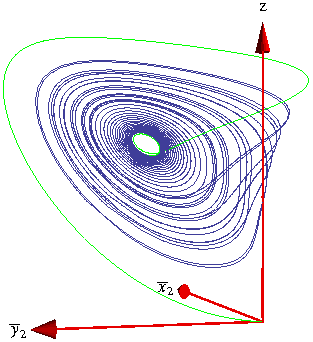
\includegraphics[width=0.35\textwidth]{CLEinvXYZ}
~~~~(\textit{b})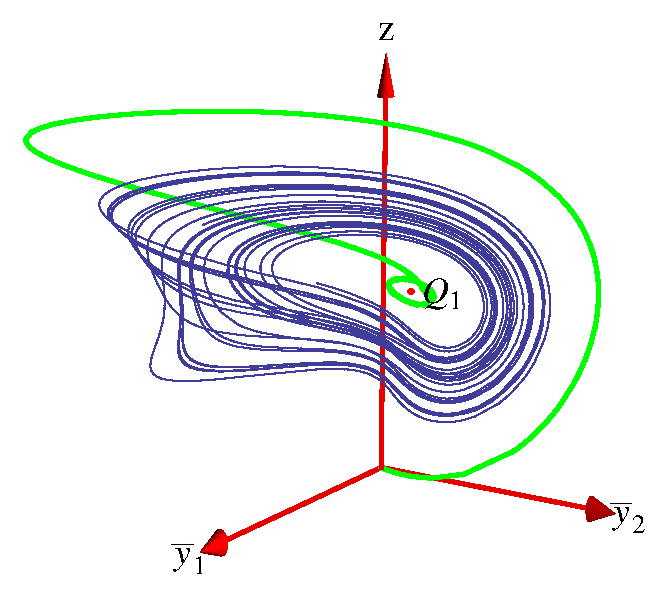
\includegraphics[width=0.35\textwidth]{CLEinvYYZ}
\end{center}
\caption{
\Statesp\ portraits of \cLe\ dynamics  in \reducedsp,
projected on invariant coordinates \refeq{eq:invLaser2}.
    }
\label{fig:CLEinv}
\end{figure}
%%%%%%%%%%%%%%%%%%%%%%%%%%%%%%%%%%%%%%%%%%%%%%%%%%%%%%%%%%%%%%%%
\ES{Fetch return map figure using unmodified invariants.}

%%%%%%%%%%%%%%%%%%%%%%%%%%%%%%%%%%%%%%%%%%%%%%%%%%%%%%%%%%%%%%%%%%
\begin{figure}[ht]
\begin{center}
%   (\textit{a})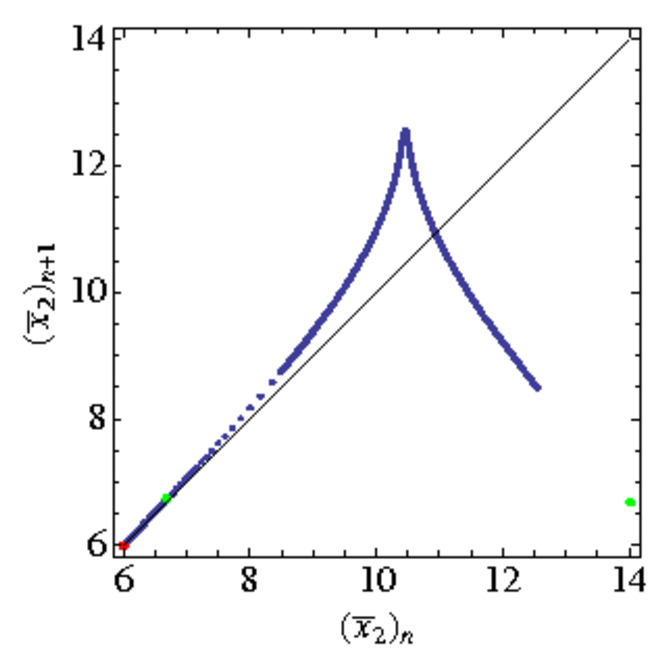
\includegraphics[width=0.35\textwidth]{CLEinvRMx2}
%  ~~~~(\textit{b})
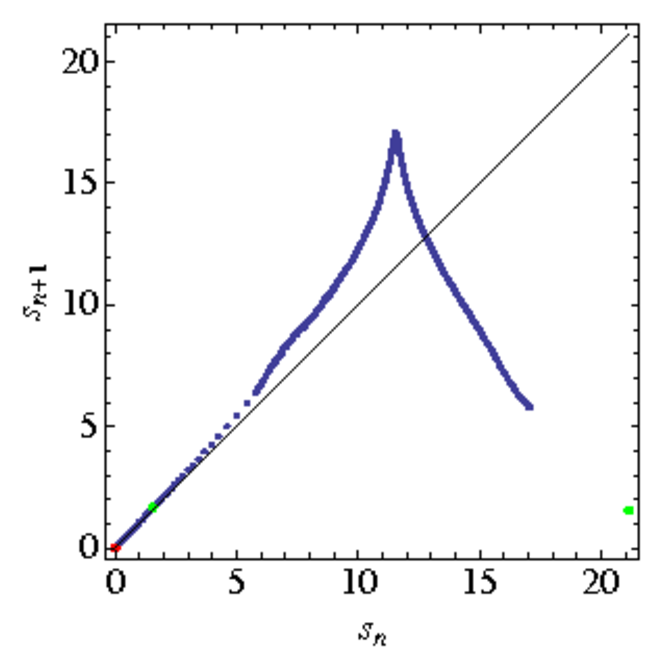
\includegraphics[width=0.35\textwidth]{CLEinvRM}
\end{center}
\caption[Return map for Complex Lorenz flow]{
Return map to the \Poincare\ surface of section
$\overline{x}_2=\overline{y}_2$ for \cLe\ with $e=1/10$,
$\ImrCLor=0$, projecting on invariants given in
\refeq{eq:invLaser2}. The return map coordinate is the
Euclidean length along the \Poincare\ section of the unstable
manifold of $E_1$.
    }
\label{fig:CLEinvRM}
\end{figure}
%%%%%%%%%%%%%%%%%%%%%%%%%%%%%%%%%%%%%%%%%%%%%%%%%%%%%%%%%%%%%%%%
} %end PublicPrivate
